\section{Evaluation in IR}\label{ch9}
\subsection{IRS quality evaluation}
In general, the evaluation of a IR system depends on two important measures: the \textbf{efficiency}, i.e. how fast the system indexes a collection and how fast it searches, and the \textbf{effectiveness/quality} of the system, which can be measured by the number of clicks in the result pages (actually not a good measure since a user suffers from many biases) or by the number of repeated visitors/buyers or the dwell time.

The most common proxy for measuring the quality of an IR system is represented by the \textbf{relevance} of the search results. In order to measure the relevance of the results, we need a \textbf{test collection} consisting of:

\begin{enumerate}
    \item A document collection;
    \item A query collection;
    \item A set of relevance judgments, standardly a binary assessment of either relevant (1) or non-relevant (0) for each query-document pair.
\end{enumerate}

The standard approach to information retrieval system evaluation revolves around the notion of \textbf{relevant} and \textbf{non-relevant} documents. With respect to a user information need, a document in the test collection is given a binary classification as either relevant or non-relevant. This decision is referred to as the gold standard or \textbf{ground truth judgment of relevance}. Notice that a document is relevant if it addresses the stated information need, not because it just happens to contain all the words in the query. 

The test document collection and suite of information needs have to be of a reasonable size: you need to average performance over fairly large test sets, as results are highly variable over different documents and information needs. In this sense, we may notice a crucial issue. Suppose that the query collection contains 50,000 queries, and that the document collection contains 5M documents: then, the matrix containing the relevance judgments would contain $0.25 \times 10^{12}$ elements, and if we suppose that each judgement takes a human 2.5 seconds, then the matrix is created in 170M hours per person. However, \textbf{crowd sourcing} can be exploited to generate such test collection.

Finally, we also need the test queries, which on the one hand must be relevant to the available documents, and on the other they must be representative of actual user needs. In general, using random query terms from the documents is not a good idea, so usually a sample from the query logs is performed, or hand-crafted queries.

\subsection{Standard test collections}
Picture \ref{tc} shows the statistic of some of the most important test collections for IR evaluation.

\begin{figure}[h!]
		\centering
		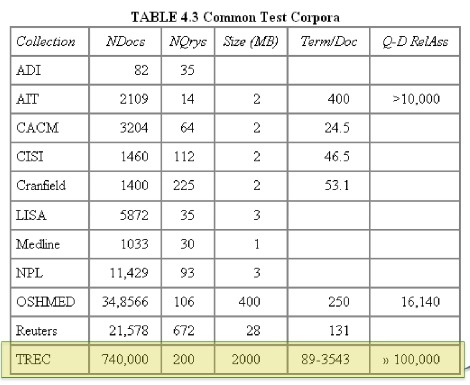
\includegraphics[scale = 1.8]{img/test collection.jpg}
		\label{tc}
        \caption{Test collections}
\end{figure}

\subsection{Evaluation of unranked retrieval sets}
The two most frequent and basic measures for information retrieval effectiveness are \textbf{precision} and \textbf{recall}. These are first defined for the simple case where an IR system returns a set of documents for a query. We will see later how to extend these notions to ranked retrieval situations.

\textit{Precision (P)} is the fraction of retrieved documents that are relevant:

$$
\text{Precision} = \frac{\text{# retrieved relevant documents}}{\text{# retrieved documents}} = P[\text{relevant} | \text{retrieved}]
$$

, while the \textit{Recall (R)} is the fraction of relevant documents that are retrieved:

$$
\text{Recall} = \frac{\text{# retrieved relevant documents}}{\text{# relevant documents}} = P[\text{retrieved} | \text{relevant}]
$$

If we consider the following contingency table

\begin{figure}[h!]
		\centering
		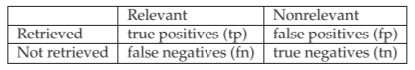
\includegraphics[scale = 2.0]{img/contingecy table.jpg}
		\label{ct}
        % \caption{Test collections}
\end{figure}

then

$$
P = \frac{tp}{tp + fp}
$$

$$
R = \frac{tp}{tp + fn}
$$

Another measure is the \textit{Accuracy}, i.e. the fraction of classification of the IR system that are correct:

$$
\text{accuracy} = \frac{tp + tn}{tp + fp + tn + fn}
$$

However, there is a good reason why \textbf{accuracy} is \textbf{not an appropriate measure} for information retrieval problems. In almost all circumstances, the \textbf{data} is \textbf{extremely skewed}: normally over 99.9\% of the documents are in the non-relevant category. A system tuned to maximize accuracy can appear to perform well by simply deeming all documents non-relevant to all queries, but labeling all documents as non-relevant is completely unsatisfying to an information retrieval system user. 

The advantage of having the two numbers for precision and recall is that one is more important than the other in many circumstances. Typical web surfers would like every result on the first page to be relevant (\textbf{high precision}) but have not the slightest interest in knowing let alone looking at every document that is relevant. In contrast, various professional searchers such as paralegals and intelligence analysts are very concerned with trying to get as \textbf{high recall as possible}. Nevertheless, the two quantities clearly \textbf{trade off} against one another: you can always get a recall of 1 (but very low precision) by retrieving all documents for all queries! \textbf{Recall} is a \textbf{non-decreasing function of the number of documents retrieved}. On the other hand, in a good system, \textbf{precision} usually \textbf{decreases} as the \textbf{number of documents retrieved is increased}. In general we want to get some amount of recall while tolerating only a certain percentage of false positives.

A single measure that trades off precision and recall if \textit{F measure}, which represents the weighted harmonic mean between the two measures:

$$
F = \frac{1}{\alpha \frac{1}{P} + (1 - \alpha) \frac{1}{R}} = \frac{(\beta^2 + 1)PR}{\beta^2 P + R}
$$

, where $\beta^2 = \frac{1 - \alpha}{\alpha}$ and $\alpha \in [0,1]$, thus $\beta^2 \in [0, \infty]$. 

The default \textit{balanced F measure} corresponds to $\alpha = 0.5$ or $\beta = 1$, and it is commonly written as $F_1$:

$$
F_1 = \frac{1}{0.5 \frac{1}{P} + 0.5 \frac{1}{R}} = \frac{2 P R}{P + R}
$$

Notice that values of $\beta < 1$ emphasize precision, while values of $\beta > 1$ emphasize recall. The choice of the \textbf{harmonic mean} resides in the fact that it always \textbf{less than or equal} to the \textbf{arithmetic mean} and the \textbf{geometric mean}, so when the values of precision and recall differ greatly, the harmonic mean is closer to their minimum than to their arithmetic mean. This is useful, for example, if we have a system that return all the documents. In this case the recall is 100\%, thus using the arithmetic mean we would get a 50\% of evaluation, while using the harmonic mean and assuming that the precision is very low, the score is 0.02\%, which is more explanatory.

\subsection{Evaluation of ranked retrieval results}
\textit{Precision}, \textit{recall}, and the \textit{F measure} are set-based measures, i.e. they are computed using unordered sets of documents. We need to extend these measures (or to define new measures) if we are to evaluate the \textbf{ranked retrieval results} that are now standard with search engines. In a ranked retrieval context, appropriate sets of retrieved documents are naturally given by the top-$k$ retrieved documents. 

\subsubsection{Precision-recall}

For each such set, precision and recall values can be plotted to give a \textbf{precision-recall curve}, such as the one shown in Picture \ref{precision recall}. 

\begin{figure}[h!]
		\centering
		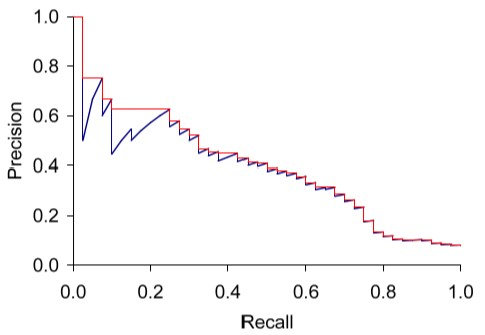
\includegraphics[scale = 2.0]{img/precision recall.jpg}
		\label{precision recall}
        \caption{Precision-recall graph}
\end{figure}

Precision-recall curves have a distinctive \textbf{saw-tooth shape}: if the $(k + 1)$-th retrieved document is non-relevant, then recall is the same as for the top-$k$ documents, but precision has dropped. If it is relevant, then both precision and recall increase, and the curve jags up and to the right. In this sense, both precision and recall increases with each relevant document retrieved, while only precision drops when a non-relevant doc is retrieved.

\subsubsection{Interpolated precision}

Since the precision-recall is not a function we consider the \textbf{interpolated precision}: the \textit{interpolated precision} $p_{interp}$ at a certain recall level $r$ is defined as the highest precision found for any recall level $r' \geq r$:

$$
p_{interp}(r) = \max_{r' \geq r} p(r')
$$

In Picture \ref{precision recall}, the \textit{interpolated precision} is depicted in red.

However, despite being very informative, there is the desire to boil the information of the \textit{interpolated precision} down to a few numbers, or perhaps even a single number. The traditional way of doing this is the \textit{11-point interpolated average precision}. For each information need, the interpolated precision is measured at the 11 recall levels of 0.0, 0.1, 0.2, . . . , 1.0. For the precision-recall curve in Picture \ref{precision recall}, these 11 values are shown in the following table:

\begin{figure}[h!]
		\centering
		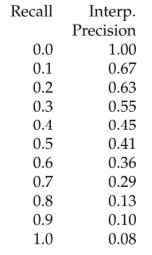
\includegraphics[scale = 1.6]{img/interpolated precision.jpg}
		\label{interpolated}
        \caption{11-point interpolated average precision}
\end{figure}

For each recall level, we then calculate the arithmetic mean of the interpolated precision at that recall level for each information need in the test collection. A composite precision recall curve showing 11 points is showed in Picture \ref{interpolated2}.

\begin{figure}[h!]
		\centering
		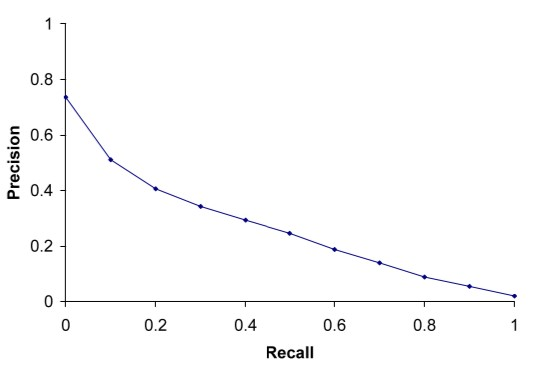
\includegraphics[scale = 1.8]{img/interpolated precision 2.jpg}
		\label{interpolated2}
        \caption{Averaged 11-point interpolated average precision across 50 queries}
\end{figure}

\subsubsection{MAP}

In recent year, other measures have become more common. One example \textbf{Mean Average Precision} or \textbf{MAP}, which has been shown to have especially good \textbf{discrimination} and \textbf{stability}. If the set of documents for a query $q_j \in Q$ is $\{ d_1, .., d_m \}$ and $R_{jk}$ is the set of ranked retrieval results from the top result until you get to document $d_k$, then:

$$
MAP(Q) = \frac{1}{|Q|} \sum_{j = 1}^{|Q|} \frac{1}{m_j} \sum_{k = 1}^{m_j} \text{Precision}(R_{jk})
$$
, i.e. it is the arithmetic mean of average precision across multiple queries/ranking.

Notice that when a relevant document is not retrieved at all, the precision value in the above equation is taken to be 0. For a \textbf{single query}, the average precision approximates the area under the uninterpolated precision-recall curve, and so the MAP is roughly the \textbf{average area under the precision-recall curve for a set of queries}. 

\underline{Example: Average Precision}

Suppose we have two rankings, as in Picture \ref{ap}, with the corresponding precision and recall.

\begin{figure}[h!]
		\centering
		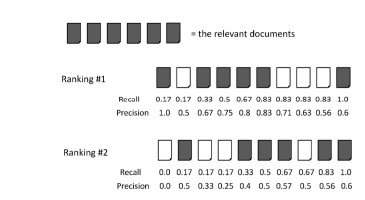
\includegraphics[scale = 2.0]{img/example AP.jpg}
		\label{ap}
        \caption{Example of AP}
\end{figure}

Then:

$$
\text{AP}_1 = (1.0 + 0.67 + 0.75 + 0.8 + 0.83 + 0.6)/6 = 0.78
$$

and 

$$
\text{AP}_2 = (0.5 + 0.4 + 0.5 + 0.57 + 0.56 + 0.6)/6 = 0.52
$$

, so both rankings retrieve all the relevant documents, but the first one has a better AP.

\underline{Example: Mean Average Precision}

Suppose we have two rankings, as in Picture \ref{map}, with the corresponding precision and recall.

\begin{figure}[h!]
		\centering
		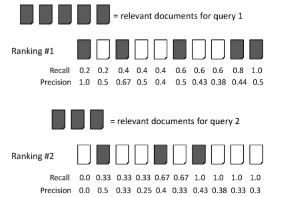
\includegraphics[scale = 2.0]{img/example MAP.jpg}
		\label{map}
        \caption{Example of MAP}
\end{figure}

Then:

$$
\text{AP}_1 = (1.0 + 0.67 + 0.5 + 0.44 + 0.5)/5 = 0.62
$$

and 

$$
\text{AP}_2 = (0.5 + 0.4 + 0.43)/3 = 0.53
$$

Finally, 

$$
\text{MAP} = (0.62 + 0.44)/2 = 0.53
$$

, so both rankings retrieve all the relevant documents, but the first one has a better AP.

\subsubsection{P@K, AP@K and MAP@K}
The above measures factor in precision at all recall levels, but for many prominent applications, particularly web search, what matters is rather \textbf{how many good results there are on the first page or the first three pages}. This leads to measuring precision at fixed low levels of retrieved results, such as 10 or 30 documents. This is referred to as \textbf{Precision@K}, e.g. Precision@10. From a mathematical point of view, the Precision@K is defined as:

$$
P@k(q_i) = \frac{1}{K} \sum_{k = 1}^K \text{rel}(q_i, k)
$$
, where 

$$
\text{rel}(q_i, k) = \begin{cases}
    1 \qquad \text{if document at rank $k$ is relevant}\\
    0 \qquad \text{otherwise}
\end{cases}
$$

\begin{figure}[h!]
		\centering
		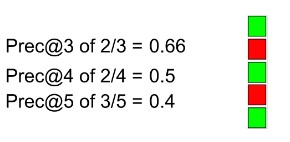
\includegraphics[scale = 2.0]{img/example prec.jpg}
		\label{prec}
        % \caption{Example of MAP}
\end{figure}

It has the \textbf{advantage} of \textbf{not requiring any estimate of the size of the set of relevant documents} but the \textbf{disadvantages} that it is the \textbf{least stable of the commonly used evaluation measures} and that it \textbf{does not average well}, since the total number of relevant documents for a query has a strong influence on Precision@k.

In a similar way, we can define AP@K as:

$$
\text{AP@K}(q_i) =  \frac{1}{K_i} \sum_{k = 1}^K P@k(q_i) \cdot \text{rel}(q_i, k)
$$
, where

$$
K_i = \sum_{k = i}^K \text{rel}(q_i, k)
$$

Finally, we can define MAP@k as:

$$
MAP@k(Q) = \frac{1}{|Q|} \sum_{q_i \in Q} AP@K(q_i)
$$

\subsubsection{MRR}
Another important measure is the \textbf{Mean Reciprocal Rank}, which is defined as follows:

$$
MRR = \frac{1}{|Q|} \sum_{i = 1}^{|Q|} \frac{1}{\text{rank}_i}
$$

, where $\text{rank}_i$ represents the rank of the first relevant document returned for a query $q_i \in Q$.

\subsubsection{DCG}
Finally, we explore the \textbf{DCG} measure. We make two assumptions:

\begin{itemize}
    \item Highly relevant documents are more useful than marginally relevant documents;
    \item The lower the ranked position of a relevant document, the less useful it is for the user, since it is less likely to be examined.
\end{itemize}

Now, this measure uses the notion of \textbf{gain} for measuring the usefulness of a document: the gain is accumulated, starting at the top of the ranking and may be reduced, or discounted, at lower ranks. If the judgements of the $n$ documents are $r_1, r_2, .., r_n$ (in ranked order), then the \textbf{cumulative gain} is 

$$
CG = r_1 + r_2 + .. + r_n
$$

In the \textbf{discounted cumulative gain}, the gain is discounted if the relevant documents appear at a rank greater than 1: a typical discount is $\frac{1}{\log(rank)}$. The DCG at a particular rank $p$ is:

$$
DCG_p = rel_1 + \sum_{i = 2}^p \frac{rel_i}{\log_2 i}
$$

An alternative formulation can be considered, where high relevance judgements become much more important:

$$
DCG@p = rel_1 + \sum_{i = 2}^p \frac{2^{rel_i}}{\log_2 (1 + i)}
$$

In this sense, this measure emphasis on retrieving highly relevant documents.

\underline{Example: DCG}

Suppose that the relevance judgements for 10 documents on a 0-3 scale are the following: [3, 2, 3, 0, 0, 1, 2, 2, 3, 0]. Then:

$$
\frac{rel_i}{\log_2 i} = [3, 2, \frac{3}{1.59}, 0, 0, \frac{1}{2.59}, \frac{2}{2.81}, \frac{2}{3}, \frac{3}{3.17}, 0] = [3, 2, 1.89, 0 , 0, 0.39, 0.71, 0.67, 0.95, 0]
$$

Then, we can compute DCG@p as:

$$
DCG@p = [3, 5, 6.89, 6.89, 6.89 , ..]
$$

\subsubsection{NDCG}
The idea of \textbf{NDCG} is to \textbf{normalize DCG} at rank $n$ by the DCG value at rank $n$ of the \textbf{ideal ranking}, where the ideal ranking would first return the documents with the highest relevance score, then the second highest etc.. 

$$
NDCG@k(Q) = \frac{1}{|Q|} \sum_{j = 1}^{|Q|} Z_{kj} \sum_{m = 1}^k \frac{2^{R(j,m) - 1}}{\log_2 (1+m)} = \frac{\text{actual DCG}}{\text{ideal DCG}}
$$
, where:

\begin{itemize}
    \item $Q$ is a set of queries;
    \item $Z_{kj}$ is a normalization factor calculated to make it so that a perfect ranking's NDCG@k for query $j$ is 1;
    \item $R(j,m)$ is the relevance score given to document $d$ for query $j$.
\end{itemize}

Notice that this normalization is particularly useful for contrasting queries with varying number of relevant documents, and for this reason it is quite popular in evaluating IR systems.

\underline{Example: NDCG}

Suppose that the perfect ranking is given by the following order of relevance judgements [3,3,3,2,2,2,1,0,0,0]. Then, the ideal DCG values would be [3, 6, 7.89, 8.89, 9.75, ..]. 

Suppose that the actual rank is [3, 2, 3, 0, 0, 1, 2, 2, 3, 0], then the actual DCG is [3, 5, 6.89, 6.89, 6.89, 7.28, ..].

Thus, the NDCG values are [1, 0.83, 0.87, ..]. Notice that $\forall k, NDCG@k \leq 1$.

\subsection{User utility}
Since the \textbf{human judgements} that are used to estimate the relevance of documents are expensive, inconsistent (both between different users and over time), and are not always a good representative of real users, we may exploit \textbf{users' clicks}. From a study we can notice that the users suffer from a strong \textbf{position bias}, i.e. they're more likely to click on links in the first position more than others, even if the link is not correct.

\subsubsection{Kendall's $\tau$}
Given a set of pairwise preferences $P$, without relevance judgements assigned to documents, we can measure the quality of two ranking $A$ and $B$ by defining a proximity measure between $A$ and $P$ and $B$ and $P$. The winning ranking is the one with better proximity with $P$. Clearly, the proximity measure should \textbf{reward} agreements with $P$, and \textbf{penalize} disagreements with $P$.

A possible proximity measure could be \textbf{Kendall's $\tau$}: let $X$ be the number of agreements between ranking $A$ and $P$, and $Y$ be the number of disagreements, then the Kendall's $\tau$ correlation between $A$ and $P$ is defined as:

$$
\tau(A,B) = \frac{X-Y}{X+Y}
$$

Notice that $0 \leq \tau(A,B) \leq 1$, and if $\tau(A,B) = 1$, then we have a perfect agreement, if $\tau(A,B) = -1$, then we have perfect disagreement, i.e. one ranking is the reverse of the other, and if $\tau(A,B) = 0$, then $X$ and $Y$ are independent.

\subsubsection{A/B testing}
If an IR system has been built and is being used by a large number of users, the system’s builders can evaluate possible changes by deploying variant versions of the system and recording measures that are indicative of user satisfaction with one variant vs. others as they are being used. This method is frequently used by web search engines. 

The most common version of this is \textbf{A/B testing}. For such a test, precisely \textbf{one thing} is \textbf{changed} between the \textbf{current system} and a \textbf{proposed system}, and a \textbf{small proportion of traffic} (say, 1–10\% of users) is randomly \textbf{directed to the variant system}, while most users use the current system. 

In IR systems, A/B testing works as follows: suppose we have two rankings for the same query, as showed in Picture \ref{ab}.

\begin{figure}[h!]
		\centering
		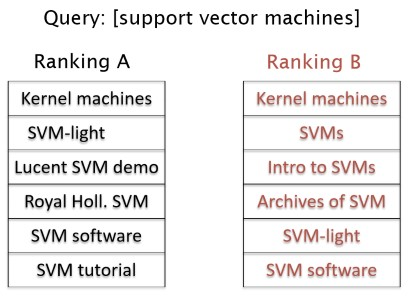
\includegraphics[scale = 2.0]{img/ab.jpg}
		\label{ab}
        % \caption{Example of MAP}
\end{figure}

We can now interleave the results of the two rankings and remove the duplicates, as shown in Picture \ref{ab1}.

\begin{figure}[h!]
		\centering
		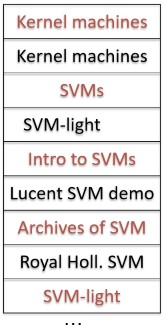
\includegraphics[scale = 2.0]{img/ab1.jpg}
        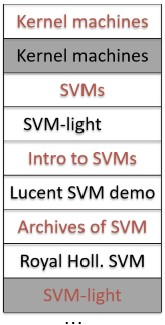
\includegraphics[scale = 2.0]{img/ab2.jpg}
		\label{ab1}
        % \caption{Example of MAP}
\end{figure}

Finally, we can count the clicks on results from A versus the results from B, as showed in Picture \ref{ab2}: better rankings will (on average) get more clicks.

\begin{figure}[h!]
		\centering
		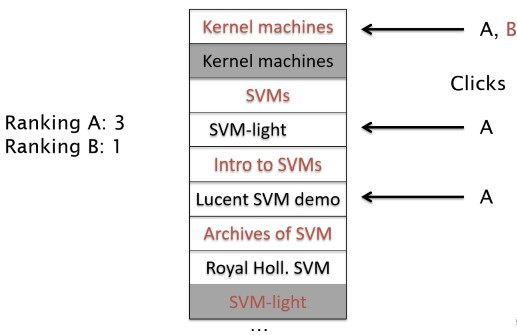
\includegraphics[scale = 2.0]{img/ab3.jpg}
		\label{ab2}
        % \caption{Example of MAP}
\end{figure}

In practice, though, A/B testing is widely used, because A/B tests are easy to deploy, easy to understand, and easy to explain to management.